%%Maximum length = smallestOf( 12,000 words, 35 pages )
%%Report file name must be "team_X.pdf" (where X is the team name)

%Your initial report set out your aims for the project which you may wish to modify in light of feedback received. The final report should detail out what you set to achieve, what you did achieve, how you achieved it, and your evaluation of your work. You are free to structure your report as you see fit, and different projects may naturally lead to different structures. An example structure for your report follows. Bear in mind that the main aim of your report is to show the examiners that you have done quality work: focus on the noteworthy, not the mundane; explain what the examiners cannot know rather than the obvious; and show that you understand your project’s weaknesses as well as its strengths.

\section{Introduction}
%Describe the context for the work and the problem you are addressing. Briefly summarise what you achieved in the project.

\begin{itemize}
	\item Context
	\item summary of chevos
\end{itemize}

\section{Review}
%Describe related work.

\begin{itemize}
    \item SUMO
\end{itemize}

\section{Requirements and Design}
%Describe the requirements you set for your project at the beginning and the design you have taken for your project. Focus on why you decided to tackle the problem in the way you did, and what effects that had on the design. You may also wish to mention the impact of team-working on your requirements and design.


\section{Implementation}
%Describe the most significant implementation details, focussing on those where unusual or detailed solutions were required. Quote code fragments where necessary, but remember that the full source code will be included as an appendix. Explain how you tested your software (e.g. unit testing) and the extent to which you tested it. If relevant to your project, explain performance issues and how you tackled them.

\subsection{Technology and libraries}
\begin{itemize}
    \item Java SE 1.8
    \item most of the actual simulation and drawing code is written manually
    \item libraries used: main code: java standard library (rt.jar), testing code: junit, mockito, fest-assert. Own logger used.
\end{itemize}


\subsection{Map data import \(OSM\)}
\begin{itemize}
    \item Map construction
    \begin{itemize}
        \item OSM xml import - as an XML file with published standard (lane directions and such)
        \item Types of data not working for us - we need  a connected graph of roads, OSM has some ways/nodes, loosely  connected (via IDs)
        \item Roads are represented as no-width polylines (no individual lanes except for just having the property)
        \item crossroads are sometimes marked nodes, sometimes just a node used in two ways.
        \item mention specifically the issue with the loosely coupled data/inaccurate data (human error, multiple representations etc.). We had to 'cut edges' to get it there.
        \item SUMO has that capability but implements its own tags and does some guess work
    \end{itemize}
\end{itemize}

\subsection{Graph construction}

\begin{itemize}
	\item Thoughts
	\begin{itemize}
		\item why construct the graph prior to the sim run instead of during	
		\item > moving the workload at startup time so as to runtime increase performance
		\item > able to conceptually save state of graph on each tick if save is implemented
	\end{itemize}
	\item Original premise: Links, Junctions and Roads

\begin{figure}
	\vspace{1.5em}
  	\caption{Original design for roads}
  	\label{fig:RoadsOriginal}
  	\centering
	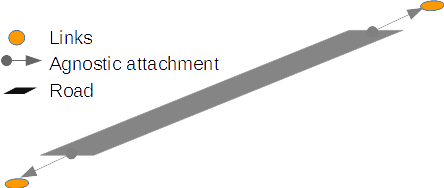
\includegraphics[width=0.55\textwidth]{figs/graphConstruction/OriginalRoads.png}
  	\vspace{1.5em}
\end{figure}	
	
	\item >>> PIC
	\item Progressed into Links, Junctions, Lanes in Directed lane group in Road
	\item > linkage done on a lane level instead of road to make it easier to construct a directed graph
	\item >>> PIC
	\item link descriptions are depreciated after work on the OSM showed that universal linkage with junctions were for easier to do then identifying what was 1-to-1 link or a junction from the OSM data
	\item Graph now composed of directed lanes -> links and Junction features with special JunctionLinks
	\item Roads are now abstracted in the graph. Lanes still belong to groups of directed lanes which, in turn, belong to roads but the graph connections are done at lane level.
	
\begin{figure}
	\vspace{1.5em}
  	\caption{Roads, Directed lane group and lanes}
  	\label{fig:RoadsFinal}
  	\centering
	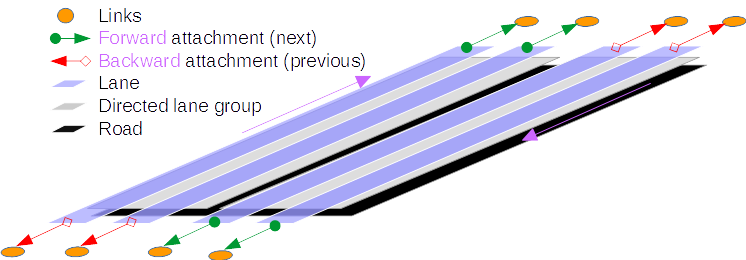
\includegraphics[width=1\textwidth]{figs/graphConstruction/Roads.png}
  	\vspace{1.5em}
\end{figure}	
	
\begin{figure}
	\vspace{1.5em}
  	\caption{Junction}
  	\label{fig:junction}
  	\centering
	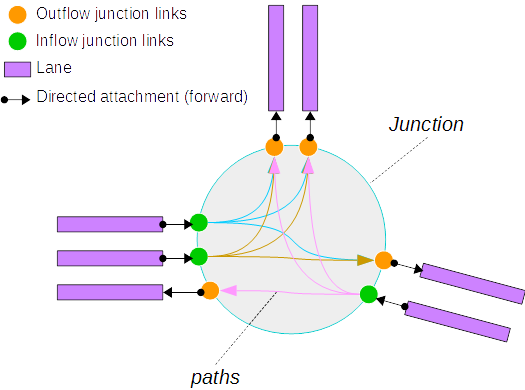
\includegraphics[width=0.6\textwidth]{figs/graphConstruction/Junction.png}
  	\vspace{1.5em}
\end{figure}		
	
	
	\item Roads and directed lane kept for keeping track of what belongs where on the simulation map. e.g.: road with name can be back referenced from a lane.
	\item 
\end{itemize}

\begin{itemize}
	\item Problems:
	\item > issues streaming from the OSM data leads to bug where in a round about a incoming road cannot be connected up
	\item > Example!! + PIC + explanation as to why exactly
\end{itemize}

\subsection{Traffic Generators}
\begin{itemize}
	\item TF originally used to produce traffic only
	\item progressed to also receive traffic exiting the boundaries of the graph
	\item keeps tab on vehicles received and produced
	\item responsible for the destruction of vehicle object
	\item Bug: incoming only lanes to a junction
	\item Bug: 1 dual way road and then all incoming composed roads into junction meant that for the incoming of the 2 way road, the traffic had no where to go.
	\item >> Both dealt with by placing TF on junctions
	\item Bug: originally linkage was checked forward only in the direction of the lanes. Not backwards. meaning if no forward lanes were present in an asymmetric road then the outgoing lanes would not get a TF connected as they were not detected.
	\item Problem fixed by introducing the "previous link" connection to all features.
\end{itemize}


\subsection{Traffic Lights}
\begin{itemize}
    \item two types of traffic lights: singles and those in one junction set
    \item all traffic lights work autonomously
	\item traffic light state: discussion whether traffic light State should be boolean or enum \(everyone wrote his version of boolean traffic lights, different ideas so we have taken Enum\)
\end{itemize}

\begin{itemize}
	\item serialization/de-serialization
\end{itemize}


\subsection{Map visualisation}
\begin{itemize}
    \item Map visualisation
    \begin{itemize}
        \item Coordinate conversion - lat/lon to meters-offset (Mercator projection). This is internal representaiton which is used in in simulation itself
        \item Coordinate conversion - meters-offset to pixels x/y (on-screen). This is the view-centric coordinate system which depends on scale, movement, size of window.
        \item Vehicle specific coordinates: lane it belongs to AND position along the polyline.
    \end{itemize}
\end{itemize}

\subsection{Vehicle movement}
\begin{itemize}
    \item Junctions and possible outcomes for vehicle
    \begin {itemize}
        \item our model: junctions 1-type: only 2 roads connected
        \item our model: junction 2-type: more than 2 roads connected (actual junctions)
        \item explain incoming lane angle, outgoing angles and its effect on vehicle movement - what is considered straight movement, and what is considered turn. >110 is prohibited, 110-30 is turn 30-0 is straight. This enforces us to skip weird turns at forks, for example.
    \end {itemize}

    \item Vehicle movement
    \begin{itemize}
        \item Straight movement on the road (even when curved). Acceleration and deceleration.
        \item Deciding if to go forward or turn (random)
        \item Crossings. Movement on 2+F crossroads (more than 2 features).
        \item Distance the car keeps to obstacles
            \begin{figure}
                \caption{Car changing lane}
                \label{fig:carKeepingDistance}
                \centering
                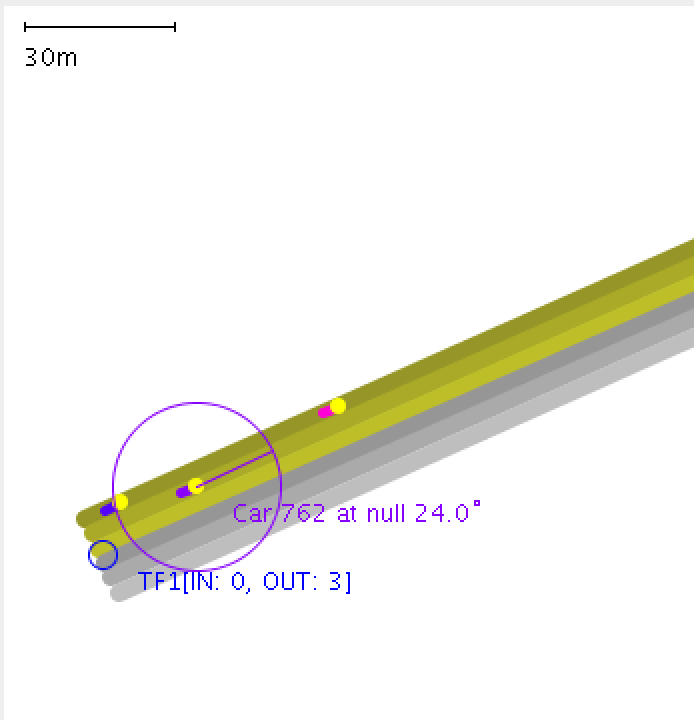
\includegraphics[width=0.3\textwidth]{figs/carMovement/car_keeping_distance_to_other.png}
                \hspace{0.2em}
                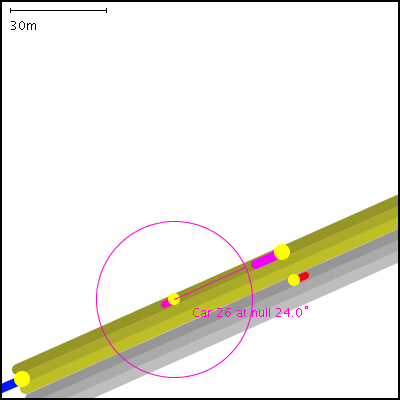
\includegraphics[width=0.3\textwidth]{figs/carMovement/car_lane_change_before.png}
                \hspace{0.2em}
                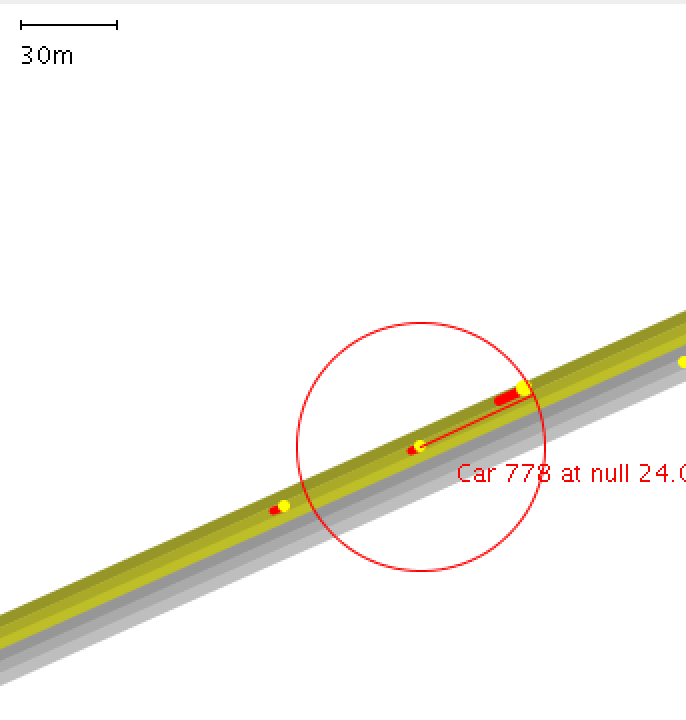
\includegraphics[width=0.3\textwidth]{figs/carMovement/car_lane_change_after.png}
            \end{figure}
        \item Lane changing - if there is another car in distance to keep, see to outer lane (if the same space is free) and change if possible, then try to do same for inner lane. If both buys, just brake.
    \end{itemize}

\end{itemize}


\subsection{Logger}
\begin{figure}
	\vspace{1.5em}
  	\caption{Logger overview}
  	\label{fig:logger_overview}
  	\centering
	\includegraphics[width=0.75\textwidth]{figs/logger/LogModuleObjectDiagram.png}
  	\vspace{1.5em}
\end{figure}

\begin{itemize}
    \item explain why and usage scenarios
    \item add basic arch. uml here
    \item Log config option injection \(why/how\)
    \item Output formats (impact on performance)
\end{itemize}

\begin{itemize}
    \item Log module
    \begin{itemize}
        \item coloured terminal window if more time,
        \item >easier to read
        \item >segregated from the console
        \item Custom Filters
        \item >filtering based on class name (origin)
        \item >filtering based on selection of multiple non-sequential log levels instead of everything below the set global level (granular control)
    \end{itemize}

     \item Traffic Lights
     \begin{itemize}
        \item traffic lights rules are basic, they do not change states according to the traffic (not intelligent traffic lights)
        \item only two states in traffic lights: red and green, we do not have early/late yellow etc.
     \end{itemize}
\end{itemize}


\section{Team Work}
%Describe how you worked together, including the tools and processes you used to facilitate group work.

    \begin{itemize}
        \item learned how to properly use team-collaborative tools
		\begin{itemize}
                \item IntelliJ Idea
                \item >facilitated git work through their embedded VCS module
                \item >Very nice code/doc and test outline generation. Enables user to focus on the important stuff instead of boilerplate code
                \item Trello
                \item >Originally used to help with Kanban process but as the updates inside and usage were sporadic and only done by some members of the group it didn't live up to its fullest potential.
                \item Hipchat
                \item > Useful for day to day communication and updates with the github/trello plug-in to keep an overview on the activities done within the group
                \item > Not everyone was diligent in being on it whilst working on the code but, when used, very useful to shout out and get quick answers to question to the members online at the time.
         \end{itemize}
         
        \item learned time-allocating in collaborative environment
        \item learned  problem solving in collaborative environment
        \item learned  conflict solving in collaborative environment
        \item NOTE> Maybe worth talking about the group marking here once that's done.
        \item Regular weekly meetings
        \item learning from each other
        \item > (JUnit tests)
        \item > Technical problems addressed - Example?
        \item > Individual strengths can be shared in a group setting
    \end {itemize}
    
    Problems:
    \begin{itemize}
    	\item procrastination and lack of pro-activity were a problem.
    	\item Extended periods of low output for the project lead to loosing track of the changes and difficulty understanding current states of the project on a technical level for some members
    	\item Other peripheral tasks (both technical and not - e.g. research, docs, report.. ) tended to be ignored or relegated to the low priority list in cases
		\item code review was not as effective as it could have been in fostering legacy learning from more experienced members due to the sporadic contribution in cases
    	\item In meetings: Code writing once the issues of the week were discussed was not as productive as it could have been during these sessions
    	\item combination of these issues lead to an asymmetric distribution of work input on the project
    \end{itemize}

\section{Evaluation}
%Critically evaluate your project: what worked well, and what didn’t? How did you do relative to your plan? what changes were the result of improved thinking and what changes were forced upon you? how did your team work together? etc. Note that you need to show that you understand the weaknesses in your work as well as its strengths. You may wish to identify relevant future work that could be done on your project.
\subsection{Possible further development}
\begin{itemize}
	\item Scaling number of cars to the size of the graph  (map)
	\item Round about issue with importing OSM data made by humans 
	\item -> allow export from other sources /API calls (gmap?)
	\item -> allow for manual editing of the graph from the GUI view?
	\item As skirting into hybrid model, detailing such as car sprites, road graphics, etc could be added as zoom factor increases, maybe show lanes from medium zoom and abstract into dots and coloured roads at low zoom
	\item addition of plug-in capability to add different metrics/behaviours as required by the user
\end{itemize}


\subsection{Performance}

\begin{center}
\begin{longtabu} to \textwidth {|
    X[2,l]|
    X[4,l]|
    X[3,c]|
    X[3,c]|
    X[3,c]|
    }
    \hline
    \textbf{Sample} & \textbf{Size} & \textbf{XML load} & \textbf{Graph linkage} & \textbf{Roads draw time} \\ \hline
Straight road & 1 road and 0 junction, 9 mapFeatures, 12 mapLinks, 2 traffic generators & 4 & 0 & 2 \\ \hline
Elephant and Castle & 101 road and 80 junction, 454 mapFeatures, 18 mapLinks, 12 traffic generators & 37 & 4 & 8 \\ \hline
Paris, Arc & 284 road and 168 junction, 1145 mapFeatures, 57 mapLinks, 35 traffic generators & 118 & 68 & 70 \\ \hline
Manhattan, Battery Park & 212 road and 148 junction, 829 mapFeatures, 81 mapLinks, 40 traffic generators & 11 & 5 & 29 \\ \hline
Strand area & 781 road and 530 junction, 2998 mapFeatures, 196 mapLinks, 105 traffic generators & 62 & 19 & 41 \\ \hline
Buckingham Palace& 275 road and 176 junction, 1032 mapFeatures, 68 mapLinks, 41 traffic generators & 28 & 8 & 21 \\ \hline
Whole Manhattan & 14763 road and 10429 junction, 58394 mapFeatures, 1055 mapLinks, 596 traffic generators & 13607 & 468 & 531 \\ \hline
Whole Greater London & 31101 road and 24314 junction, 120672 mapFeatures, 547 mapLinks, 391 traffic generators & 32911 & 644 & 1087 \\ \hline

\end{longtabu}
\end{center}
All time units in milliseconds.

Alex: probably worth making these numbers up to a nice table, wdyt?

Test machine: OS X, Intel Core I7-4770HQ, 2.2 GHz, 16GB RAM, SSD


\section{Peer Assessment}
%In a simple table, allocate the 100 ‘points’ you are given to each team member. Valid values range from 0 to 100 inclusive. You may assign decimal values, but the entire points must add up to precisely 100.

 \begin{itemize}
        \item Kumar Awijeet
		\item Oleksandr Cherednychenko
		\item Esmond A. Davison
		\item Jacek Krupski
		\item Farhad Rahimli
    \end{itemize}
